\section{Numerical implementations}
\subsection{Cutting the cell with $\alpha$ and $\phi$}
In this case, the normal direction $\mathbf{n}$ of certain cell is given by level set function $\phi$ and the void fraction $\alpha$ is given by volume of fluid function. This section means to explain the algorithm of finding such a plane with normal direction $\mathbf{n}$ that can cut the cell into the right void fraction $\alpha$. The locations of cell center point $\mathbf{x_i}$ and $N$ cell vertexes $\mathbf{x_{i_1}},...,\mathbf{x_{i_N}}$ are needed. Then we can get $N$ vectors $\mathbf{d_1},...,\mathbf{d_N}$ from cell center to $N$ cell vertexes. The projections of center point to vertex on the normal direction can be calculated as
\begin{equation}\label{21}
D_i=\mathbf{d_i}\cdot\mathbf{n},\quad for\quad i=1,...,N.
\end{equation}
Let us suppose the objective plane contain one of the vertexes and we can have a series of plane to cut the cell into different fractions (figure \ref{fig:multiplane}). Due to the cell's polyhedral characteristic, a piecewise function about the center cell distance and void fraction is drew in figure \ref{fig:piecewise}. The objective plane with the given void fraction $\alpha_i$ must have a certain distance $D^*$ to the center point $\mathbf{x_i}$ such that $\tilde{\alpha}(D^*)=\alpha_i $ .The first step is to find the point on the certain part of the piecewise function, which can be realized by comparing the void fraction value of vertexes and $\alpha^*$. Suppose the point $p$ is between point $k$ and $l$, such that ${D^*}\in[D_k,D_l]$. We use a cubic polynomial to fit this interval. The second step is to find the two trisection point in this interval, say, $m$ and $n$, and calculate the $\tilde{\alpha}(D_m)$ and $\tilde{\alpha}(D_n)$ in geometric way. Then we have four points for the four polynomial coefficients by solving a group of linear equations. Use LU decomposition to solve the linear $4\times4$ Vandermonde matrix system. Then use Newton's root finding method to find $D^*$ with the condition, $\left|\tilde{\alpha}(D^*)-\alpha_i\right|<\epsilon$. $\epsilon$ is a user-defined tolerance, typically set to $10^{-8}$.

\begin{figure}[htbp]
\centering
\subfigure[]{
\centering
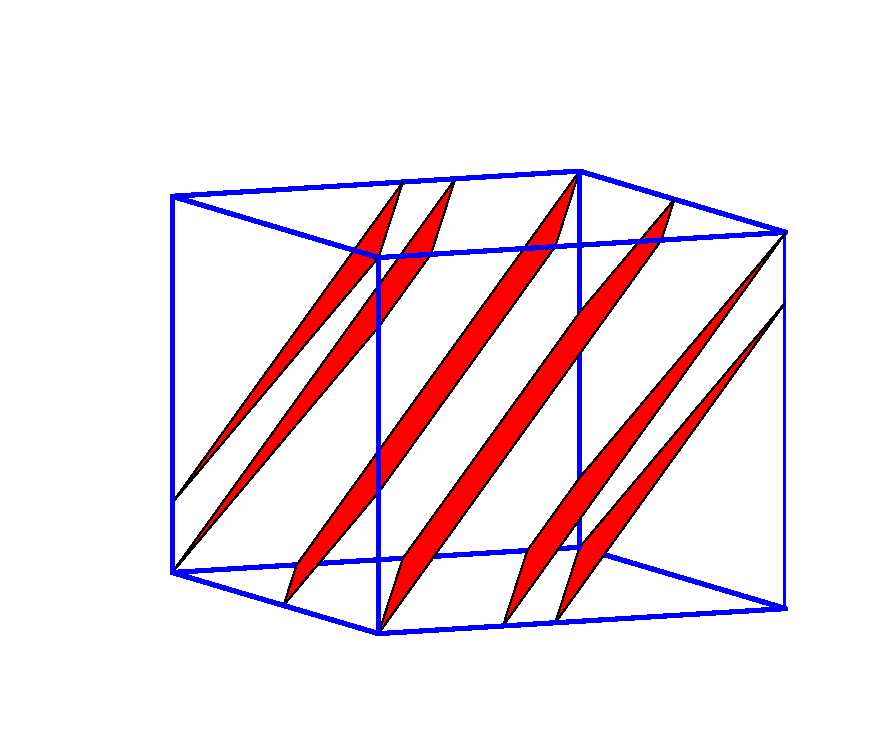
\includegraphics[width=0.4\textwidth]{multiplane.eps}
%\caption{fig1}
\label{fig:multiplane}
}
\quad
\subfigure[]{
\centering
\includegraphics[width=0.4\textwidth]{piecewisefunction.eps}
\label{fig:piecewise}
%\caption{fig2}
}
%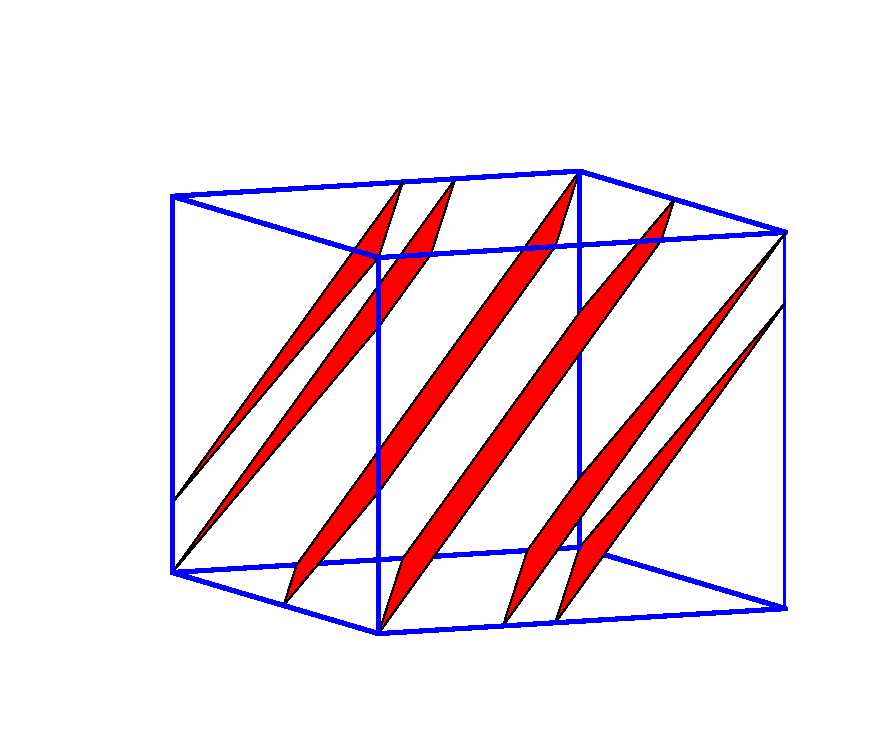
\includegraphics [width=0.5\textwidth]{multiplane.eps}
\caption{\subref{fig:multiplane} shows that planes pass different vertexes with the same normal direction. \subref{fig:piecewise} shows the cut volume and distance to the plane.}
\label{fig:multi}
\end{figure}

\subsection{Narrow band containing interface}
The cells that contain the interface are limited to where $H\in(\xi,1-\xi)$. $\xi$ is defined by users to confine the algorithm resolution, usually set as $0.0001$. The reason why uses Heaviside function rather than void fraction is that the interface defined by Heaviside function is more explicit and void fraction function more smeared. However, only interface cells are not enough to reconstruct the details of the interface. Level set method needs to build the signed distance function in the whole field, which can precisely capture the interface. Nonetheless, it takes too much computational resource and time to calculate on the whole field. So it is necessary to build a narrow band that has a thickness of two layers of grid like figure(\ref{fig:NarrowBand}). The first step is to sign all the interface cells with the flag "seed" and all the non-interface cell with the flag "away". The second step is to find the cells that share the vertexes of the "seed" cell. If the cells are signed with flags including "away" or "second layer", sign them with the flag "first layer". The third step is to traverse the cells that share the vertexes of the "first layer" cells. If the cells are signed with flags "away", sign them with the flag "second layer". Thus the narrow band that contains the interface and two-layers grids is built. The Heaviside function field and normal direction vector field can be limited in the narrow band to evade unnecessary computation.
\begin{figure}[htbp]
\centering
\includegraphics[width=0.5\textwidth]{band.eps}
\caption{The numbers in cells mean the flag. 0: "seed", 1:"first layer", 2:"second layer" and 4:"away"}
\label{fig:NarrowBand}
\end{figure}

\subsection{Reinitialization}

\subsection{Correction for mass conservation}

\subsection{Numerical Discretization of level set equation}

